% Options for packages loaded elsewhere
\PassOptionsToPackage{unicode}{hyperref}
\PassOptionsToPackage{hyphens}{url}
%
\documentclass[
]{book}
\usepackage{amsmath,amssymb}
\usepackage{iftex}
\ifPDFTeX
  \usepackage[T1]{fontenc}
  \usepackage[utf8]{inputenc}
  \usepackage{textcomp} % provide euro and other symbols
\else % if luatex or xetex
  \usepackage{unicode-math} % this also loads fontspec
  \defaultfontfeatures{Scale=MatchLowercase}
  \defaultfontfeatures[\rmfamily]{Ligatures=TeX,Scale=1}
\fi
\usepackage{lmodern}
\ifPDFTeX\else
  % xetex/luatex font selection
\fi
% Use upquote if available, for straight quotes in verbatim environments
\IfFileExists{upquote.sty}{\usepackage{upquote}}{}
\IfFileExists{microtype.sty}{% use microtype if available
  \usepackage[]{microtype}
  \UseMicrotypeSet[protrusion]{basicmath} % disable protrusion for tt fonts
}{}
\makeatletter
\@ifundefined{KOMAClassName}{% if non-KOMA class
  \IfFileExists{parskip.sty}{%
    \usepackage{parskip}
  }{% else
    \setlength{\parindent}{0pt}
    \setlength{\parskip}{6pt plus 2pt minus 1pt}}
}{% if KOMA class
  \KOMAoptions{parskip=half}}
\makeatother
\usepackage{xcolor}
\usepackage{longtable,booktabs,array}
\usepackage{calc} % for calculating minipage widths
% Correct order of tables after \paragraph or \subparagraph
\usepackage{etoolbox}
\makeatletter
\patchcmd\longtable{\par}{\if@noskipsec\mbox{}\fi\par}{}{}
\makeatother
% Allow footnotes in longtable head/foot
\IfFileExists{footnotehyper.sty}{\usepackage{footnotehyper}}{\usepackage{footnote}}
\makesavenoteenv{longtable}
\usepackage{graphicx}
\makeatletter
\def\maxwidth{\ifdim\Gin@nat@width>\linewidth\linewidth\else\Gin@nat@width\fi}
\def\maxheight{\ifdim\Gin@nat@height>\textheight\textheight\else\Gin@nat@height\fi}
\makeatother
% Scale images if necessary, so that they will not overflow the page
% margins by default, and it is still possible to overwrite the defaults
% using explicit options in \includegraphics[width, height, ...]{}
\setkeys{Gin}{width=\maxwidth,height=\maxheight,keepaspectratio}
% Set default figure placement to htbp
\makeatletter
\def\fps@figure{htbp}
\makeatother
\setlength{\emergencystretch}{3em} % prevent overfull lines
\providecommand{\tightlist}{%
  \setlength{\itemsep}{0pt}\setlength{\parskip}{0pt}}
\setcounter{secnumdepth}{5}
\usepackage{booktabs}
\usepackage{amsthm}
\makeatletter
\def\thm@space@setup{%
  \thm@preskip=8pt plus 2pt minus 4pt
  \thm@postskip=\thm@preskip
}
\makeatother
\ifLuaTeX
  \usepackage{selnolig}  % disable illegal ligatures
\fi
\usepackage[]{natbib}
\bibliographystyle{apalike}
\usepackage{bookmark}
\IfFileExists{xurl.sty}{\usepackage{xurl}}{} % add URL line breaks if available
\urlstyle{same}
\hypersetup{
  pdftitle={Tutorial on Phonetics and Speech Analysis},
  hidelinks,
  pdfcreator={LaTeX via pandoc}}

\title{Tutorial on Phonetics and Speech Analysis}
\author{true \and true}
\date{Document compiled 17 Nov 2024 14:48}

\begin{document}
\maketitle

{
\setcounter{tocdepth}{1}
\tableofcontents
}
\chapter*{Preface}\label{preface}
\addcontentsline{toc}{chapter}{Preface}

\section*{Aims}\label{aims}
\addcontentsline{toc}{section}{Aims}

In this tutorial you will learn about \textbf{acoustics} (sounds), \textbf{phonetics} (speech), and \textbf{speech analysis}.
You will learn the core concepts in these related fields, as well as the necessary practical skills for speech analysis.
The aim of this tutorial is to provide you with the phonetic insights and skills in speech analysis that you need to succesfully conduct phonetic research in your own project (e.g.~paper or thesis).

\subsection*{Under construction}\label{under-construction}
\addcontentsline{toc}{subsection}{Under construction}

This tutorial is a work in progress, resulting from an ongoing revision of an existing tutorial, and meanwhile incorporating other modules and resources.

The existing (outdated) full tutorial is still available at \url{https://resources.lab.hum.uu.nl/resources/phonetics/index.html}
.

More details on the origins of this tutorial are provided below.

\section*{How to use this tutorial}\label{how-to-use-this-tutorial}
\addcontentsline{toc}{section}{How to use this tutorial}

You will learn the most from this tutorial if you

\begin{enumerate}
\def\labelenumi{(\arabic{enumi})}
\tightlist
\item
  read the explanatory texts in this tutorial,
\item
  work through the questions and exercises provided,
\item
  practice in applying your new knowledge hands-on, with the \texttt{Praat} computer program (detailed below), and
\item
  re-read the relevant sections from this tutorial and your textbook, with the help of keywords provided per section.
\end{enumerate}

\phantomsection\label{question-intro}
\subsection*{Questions}\label{questions}
\addcontentsline{toc}{subsection}{Questions}

Text blocks such as this one will contain questions or exercises inviting you to engage with the tutorial. You will learn most if you attempt to answer these questions (preferably in writing) \emph{before} you proceed and \emph{before} you take a look at the answer provided. (These questions only work in the HTML version of the tutorial; other versions will just show both the question and answer subsequently.)

\subsubsection*{Question 0.1}\label{question-0.1}
\addcontentsline{toc}{subsubsection}{Question 0.1}

What is sound?

Answer 0.1

Sound is a type of energy that travels through a medium (such as air, water, or solid materials) in the form of waves. These sound waves are created by the vibration of objects, which causes the surrounding particles in the medium to move in a back-and-forth motion. This movement, or vibration, transfers energy through the medium, creating waves of high and low pressure.

\section*{Recommended software}\label{recommended-software}
\addcontentsline{toc}{section}{Recommended software}

In this tutorial you will work mostly with \texttt{Praat} \citep{Boersma_Weenink_2024}\footnote{The Dutch word \emph{praat} /ˈpraːt/ means ``talk''.}. This is a popular open-source program for the analysis of speech, developed by Paul Boersma and David Weenink (both at University of Amsterdam). It can be found on its own website (\url{https://www.praat.org}), where you will find a wealth of helpful documentation. \texttt{Praat} also has extensive \texttt{Help} built in, including a full tutorial.\\
There is an online forum (\url{https://groups.io/g/Praat-Users-List}), where users share their knowledge by posting questions and providing answers.

In order to install \texttt{Praat} on your computer, go to its webpage at \url{https://www.praat.org/}, and then proceed to the download page for the operating system of your computer. Follow the installation instructions on the download page for your operating system.

\phantomsection\label{tech-layout}
\subsection*{\texorpdfstring{Instructions for using \texttt{Praat}}{Instructions for using Praat}}\label{instructions-for-using-praat}
\addcontentsline{toc}{subsection}{Instructions for using \texttt{Praat}}

Text blocks such as this one will contain instructions about how to ``do'' things in \texttt{Praat}.

Options in software menus, as well as texts in on-screen buttons, will be shown \texttt{in\ this\ way}.
The notation \texttt{Main\ \textgreater{}\ Sub} means: first choose option \texttt{Main} from the main menu, after which a submenu will appear, then choose option \texttt{Sub} from the submenu.
Commands or formulas that you have to type will be shown \texttt{in\ this\ way} too. (Commands typically need to be terminated with typing \texttt{Enter} or \texttt{Return} or \texttt{␍} or \texttt{⏎} -- which however will not be specified in the instructions.)

\section*{Structure of this tutorial}\label{structure-of-this-tutorial}
\addcontentsline{toc}{section}{Structure of this tutorial}

TBA

\section*{Recommended textbooks}\label{recommended-textbooks}
\addcontentsline{toc}{section}{Recommended textbooks}

This tutorial is intended to be used in addition to one or more textbook(s) in Phonetics, to which this tutorial will provide additional background knowledge. Some excellent textbooks in Phonetics are those by
\citet{Rietveld_VanHeuven_2009} (in Dutch),
\citet{Johnson_2011},
\citet{Ladefoged_Johnson_2015},\\
\citet{Reetz_Jongman_2020}, and
\citet{Zsiga_2024}.

\section*{Details}\label{details}
\addcontentsline{toc}{section}{Details}

\subsection*{License}\label{license}
\addcontentsline{toc}{subsection}{License}

This work is licensed under the \emph{GNU GPL 3} license (for details see
\url{https://www.gnu.org/licenses/gpl-3.0.en.html}).

\subsection*{Citation}\label{citation}
\addcontentsline{toc}{subsection}{Citation}

TBA

\subsection*{Technical details}\label{technical-details}
\addcontentsline{toc}{subsection}{Technical details}

TBA

\subsection*{History}\label{history}
\addcontentsline{toc}{subsection}{History}

This work is based on an earlier tutorial (2006-2007) titled Tutorial for self study: basics of phonetics and how to use Praat by Clizia Welker and Hugo Quené. In turn, that 2007 tutorial was partly based on older texts by Hugo Quené, Denise Bruin and Mirjam Wester (1996-2000); these older texts acknowledged valuable comments and suggestions by Paul Boersma, Olga van Herwijnen, Kim Koppen, Eva Sittig, Joyce Vliegen and Mieke van Wijck.

The 2007 version of the tutorial was subsequently revised and adapted to the current version using \texttt{R\ Markdown} \citep{rmarkdown2018} and \texttt{bookdown} \citep{R-bookdown} in \href{https://www.rstudio.com}{Rstudio} by Hugo Quené in 2024.

\begin{center}\rule{0.5\linewidth}{0.5pt}\end{center}

\part*{Part I: Sounds}\label{part-part-i-sounds}
\addcontentsline{toc}{part}{Part I: Sounds}

\chapter{Sound waves}\label{ch-soundwaves}

\emph{Chapter keywords}: sound, sound wave, oscillation, propagation, longitudinal wave, transverse wave, medium, speed of sound, force, pressure, Pascal, oscillogram, frequency, Hertz, period, amplitude, intensity, phase, Pascal, \texttt{Praat}, object, visualization, picture, figure.

\section{Sound}\label{sound}

Sound is a type of energy that travels through a medium (such as air, water, or solid materials) in the form of waves. These sound waves are created by the vibration of objects, which causes the surrounding particles in the medium to move in a back-and-forth (oscillatory) motion. This movement, or vibration, or oscillation, transfers energy through the medium, creating waves of high and low pressure.

\section{Sound wave}\label{sec:soundwave}

A sound wave consists of pressure fluctuations caused by the molecules of the acoustic medium crowding together (compression) and moving apart (rarefaction). A sound wave is spread in all directions from the sound source; we could compare its propagation to that of a circular wave on the surface of a water basin. The molecules themselves move over a very short distance and do not travel along with the wave: instead, after the sound wave (the pressure fluctuation) has passed along, they go back to their equilibrium position.

Sound in air is different from wind. In wind, or in air flow, the air particles move from one position to another (from equator to tropics, from lungs to mouth). In sound, however, there is no net movement of the air particles: the particles only move over a very small distance, and return to their equilibrium after the sound wave has passed. In sound waves, the distance of travel of the air molecules is only about \(10^{-11}\) to \(10^{-5}\) m, depending on the amplitude and frequency of the vibration (more about these key properties in §\ref{sec:keypropertiessound} below).

There are two kinds of waves (also depending on the acoustic medium). In \emph{longitudinal} waves (such as sound waves) the back-and-forth displacement or movement of the medium's particles is in the same direction as the propagation of the wave. In \emph{transverse} waves (such as the waves on the surface of a pond) the back-and-forth displacement of the water particles is perpendicular to the direction of propagation of the wave.\\
A stadium wave provides a clear example of a transverse wave: a group of persons (the particles) starts the wave by standing up, rising their arms, sitting down, standing up again, and so on. The persons' action is directly followed by that of their neighbours on one side, who do the same and who are again followed by their next neighbours on their side, and so on, until the wave is travelling through the whole stadium. The persons' motion (up-down) is perpendicular to the propagation of the wave (left-right along the bench).

Sound propagates in all dimensions through an acoustic medium, like an expanding sphere, which is indeed the theoretical model used to describe the sound wave propagation pattern. As the sound wave moves away from its source, more particles are involved in the pressure fluctuations. As a consequence, sound waves lose energy while travelling through the medium, as some of the energy is spent in moving increasingly more particles. Finally, sound is perceived as such when the sound wave spread by the sound source and travelling through the acoustic medium finally impinges upon the eardrum of the observer.

\section{Acoustic media}\label{acoustic-media}

Air is only one of the media through which sound can propagate. If your head is under water (as in a bath, pool, lake or sea), the water may carry sound waves from the sound source to your eardrums, and you do hear sounds. The propagation of sound waves is faster through liquids than through gases such as air: the closer the molecules of the medium (i.e.~the higher its density), the higher the speed of sound in that medium.

You can also put your ear to the ground in order to hear sounds propagated through the soil. The propagation of sound waves in solid soil is even faster than in liquids. Trying this out on dry sand on the beach, one observer noted hearing footsteps until about 25 m distant \citep[§10]{Minnaert_1970v2}.

\section{The speed of sound}\label{sec:speedofsound}

In air, the speed of sound (the speed of propagation of a sound wave, symbol \(c\)) is about 332 m/s at 0°C, about 343 m/s at 20°C, and 353 m/s at at 37°C \citep{Shadle_2010} (all for dry air at sea level).
The speed of sound in a gas such as air is affected by only two parameters:
- the ambient temperature of the gas (as shown in the numbers above),
- the composition of the gas (its mixture and the density and compressibility of its component gases), including its relative humidity: humid air holds more particles (of water), resulting in a slight increase of the speed of sound as relative humidity increases \citep{Harris_1971}\footnote{For relative humidity \textgreater30\% \citep{Harris_1971}.}.

In sea water, sound travels at about 1435 m/s, in concrete 3400 m/s, in iron (e.g.~railroad tracks) about 5100 m/s.

\section{Pressure}\label{pressure}

Pressure is the amount of force on a surface. In physics, \emph{force} is defined as an influence causing an object to accelerate. It is expressed in Newton units; a Newton is the amount of force that increases the velocity of a 1-kilogram object by one meter per second (\(m/s\)). \emph{Pressure}, in turn, is defined as force per unit of area. It is measured in Pascal units, which correspond to Newton (N) per square meter (\(1\ Pa = 1\ N/m^2\)).
Under normal conditions, atmospheric air pressure is centered at 1013.25 hPa (101325 Pa, an average value\footnote{This is the standard unit of 1 atmosphere. The pressure is due to the Earth's gravition force on the Earth's atmosphere.} on a medium latitude at sea level, at 0°C), with normal meteorological fluctuations of about ± 5000 Pa. Sound wave fluctuations in air pressure are far smaller, ranging from about ±20 µPa (micropascal, or ±0.00002 Pa) at the lower threshold of hearing to about ±20 Pascal at the upper threshold of hearing. Even louder sounds, with variations in air pressure exceeding about ±20 Pascal, are painful and cause hearing damage.

\phantomsection\label{questions-soundwaves}
\section*{Questions}\label{questions-1}
\addcontentsline{toc}{section}{Questions}

\subsection*{Question 1.1}\label{question-1.1}
\addcontentsline{toc}{subsection}{Question 1.1}

Explain why a sound wave loses energy the further it is spread from the oscillation source.

Answer 1.1

The more a sound \emph{wave} moves away from the source, the more particles of the medium (e.g.~air) are involved. The amount of initial energy (spread with the source oscillation) is spread over a larger surface, of an expanding imaginary sphere, and consequently the sound wave displaces more particles. The overall amount of energy remains the same. Therefore, the energy on a single medium particle or on a single portion of the sound wave is smaller. Thus, the sound wave fades as the distance to the sound source increases.

Remember that the sound \emph{wave} travels through the medium, but the particles in the medium remain more or less in place.

\section{Oscillogram}\label{sec:oscillogram}

As explained in §\ref{sec:soundwave} above, a sound wave consists of pressure fluctuations caused by the molecules of the acoustic medium crowding together (compression) and moving apart (rarefaction). These oscillations in air pressure can be measured and visualized. (In chapter \ref{ch-soundtobytes} we'll learn how to measure, record and store a sound wave.) Here, we jump ahead and present a graphical representation of a sound wave: the \textbf{oscillogram}.
(We need the oscillogram to explain important properties of sound waves.)

In an oscillogram, the horizontal axis represents the time dimension, and the vertical axis represents the air pressure. The air pressure fluctuations (compression and rarefaction) are displayed here as vertical deviations relative to the horizontal baseline\footnote{The baseline represents the ambient average air pressure. By convention, higher air pressure is on the top side and lower air pressure at the bottom side of an oscillogram.}.
Thus an oscillogram records the back-and-forth movements of the air particles, indirectly, by recording the fluctuations in relative air pressure, at a fixed location.

\begin{figure}

{\centering 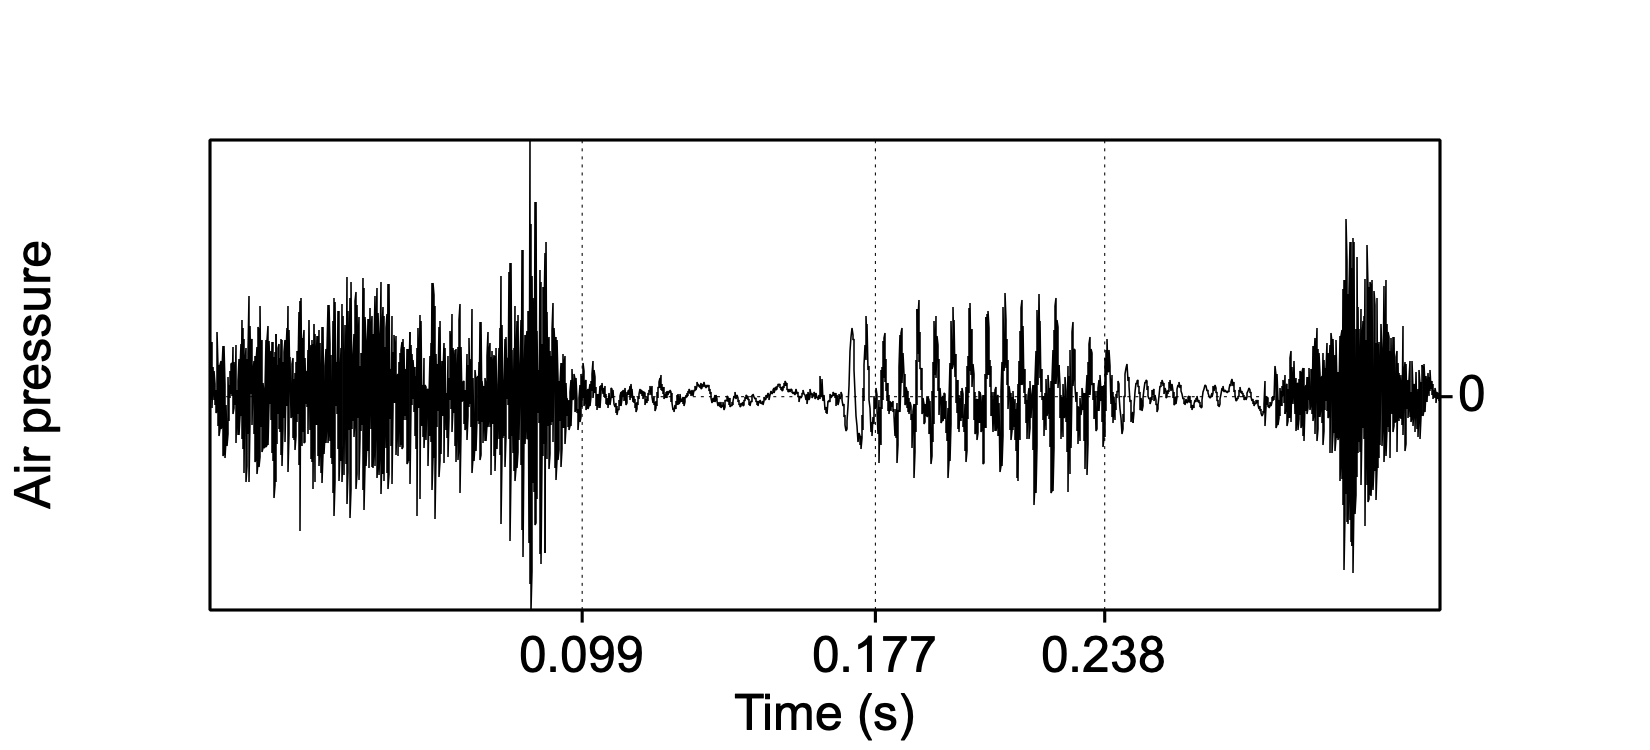
\includegraphics{figures/speech_word_oscillogram} 

}

\caption{Oscillogram of the word *speech*, with boundaries between segments.}\label{fig:speech-oscillogram}
\end{figure}

An oscillogram is comparable to a meteorologist's regular measurements of atmospheric air pressure at a fixed location --- albeit on far finer scales of time and of air pressure.

The visualisation in an oscillogram may suggest, misleadingly, that the air particles themselves dance ``up and down'' (transverse) while the sound wave travels ``from left to right'', like waves on the surface of a body of water. That is not true: sound in air travels in \emph{longitudinal} sound waves, resulting in the air pressure variations that are visualized in the oscillogram.

\section{Periodic and aperiodic sounds}\label{periodic-and-aperiodic-sounds}

There are two classes of sounds which are easily distinguishable in an oscillogram:

\begin{itemize}
\item
  \textbf{periodic} sounds, in which there is sound wave pattern that repeats itself after a particular time interval or \textbf{period} (symbol \(T\)) of a single cycle. Periodic sounds have a perceptible pitch or tone. Vowel sounds such as the /i/ in Figure \ref{fig:speech-oscillogram} (from 0.177 to 0.238 s) provide clear examples of a periodic sound.
\item
  \textbf{aperiodic} sounds, in which there is not a repetitive but instead a random pattern in the air pressure variations. Aperiodic sounds do not have a perceptible pitch but instead we hear them as noise. Some consonant sounds, e.g.~the /s/ in Figure \ref{fig:speech-oscillogram} (from 0 to 0.099 s), are clear examples of such noisy, aperiodic sounds\footnote{The clearest examples are provided by unvoiced fricative consonants, such as /f, s/.}.
\end{itemize}

\section{Key properties of a sound wave}\label{sec:keypropertiessound}

\begin{quote}
TODO: Bridging intro text.
\end{quote}

\begin{quote}
TODO: insert here an oscillogram of a periodic sound wave,
illustrating the subsequent properties in the time domain, at a fixed position in space (microphone position).
\end{quote}

\subsection{Frequency}\label{sec:frequency}

The frequency (symbol \(f\)) of a sound wave is the number of repeated cycles or periods (of air pressure variations) within a time interval. Only periodic sounds do have such repetitions, and thus a frequency. The frequency of a sound is perceived as its \emph{pitch} or tone. Frequency is expressed in periods per second, or Hertz units, named after Heinrich Rudolf Hertz (1857--1894)\footnote{In older texts you may find `cycles per second', abbreviated `cps'.}.
Each of these periods or cycles corresponds to the repeating fluctuation between two consecutive maxima, or between corresponding `zero crossings' of adjacent periods. In Figure \ref{fig:speech-oscillogram}, in the vowel /i/, we count 14 periods in 0.065 seconds, so \(f \approx 14/0.065 \approx 215\) Hz. These periods have a duration of about \(T \approx 0.065/14 \approx 0.0046\) s\footnote{More exactly, the period \emph{is} 0.0046 s.}. Period \(T\) and frequency \(f\) are each other's inverse, so \(f=1/T\) and \(T=1/f\).

In the transverse stadium wave, the period \(T\) is the time interval between two consecutive actions of standing up by the same person (e.g.~\(T=5\) s), and frequency \(f\) is the number of actions that occur within a given time unit (e.g.~\(f=1/T=1/5\) Hz).

\subsection{Amplitude}\label{sec:amplitude}

The amplitude (symbol \(A\)) of a sound wave is the extent of the variations in air pressure (due to compression and rarefaction), measured in Pascal units of pressure. With some simplification, the amplitude of a sound wave is perceived as its \emph{loudness} or `volume'. In an oscillogram, the amplitude corresponds directly to the maximum vertical displacement, that is, to the peak deviation in air pressure relative to the ambient reference pressure).

In the transverse stadium wave, the amplitude could be thought of as the extent to which persons raise their hands.

In practice, the amount of energy in a (longitudinal) sound wave is better assessed in the form of \emph{intensity}, which will be discussed in §XXX below.

\subsection{Phase}\label{sec:phase}

The phase of a sound wave (symbol \(\varphi\)) is the starting time of a sound wave period, relative to the duration of that period. It's easiest to explain by comparing two sounds. When listening, a single sound will arrive at our two ears at slightly different arrival times. (Unless the sound source is directly in front of us, the sound will have a slightly longer path to travel to the further ear than to the closer ear.) Thus the two sounds heard by the two ears will differ in phase: the starting time of a period in one ear will differ slightly from the starting time of a period in the other ear, and the difference can be expressed as the proportion of a period by which they differ.\\
The brain of the listener uses this phase difference between the two ears to estimate the direction of the sound source relative to the head. You may appreciate the effect by listening to music in mono or in stereo.

In addition, we use phase unconsciously to assess atmospheric and acoustic conditions. For example, when listening to a sound in a room, we hear not only the direct sound but also the indirect reflections from the floor, walls, ceiling, furniture, etc. The brain uses the phase relations among multiple reflections to assess the dimensions and conditions of the room.

Phase is expressed relative to the period \(T\), but it is not expressed in time (seconds) but in proportions, often expressed as degrees in the period cycle (which runs from \(0^\circ\) to \(360^\circ\)). So, a phase difference of \(\varphi=180^\circ\) and \(\varphi=0.5\) mean the same: the time difference between the two signals is half a period, whatever the duration of that period is.

In the transverse stadium wave, phase corresponds to the difference in time between the sit-down-moment of one group of persons, and the comparable sit-down-moment of another group of persons in a different section of the stadium. Imagine two waves rolling along the stadium benches: one wave on the lower benches, and a different wave on the upper benches. The two waves may be out of phase (lower and upper persons sit down at different times) or in phase (lower and upper person sit down at the same time) -- irrespective of whether the two waves have the same or different frequencies.

\phantomsection\label{questions-phase}
\subsection*{Question 1.2}\label{question-1.2}
\addcontentsline{toc}{subsection}{Question 1.2}

Continue this thought experiment, with two stadium waves having the same frequency on the lower and upper benches, and with phase \(\varphi=0.5\) between the lower and upper sections. What would the resulting wave pattern look like?

No answer provided

No answer provided\ldots{} think this out\ldots{}

\subsection{Wavelength}\label{sec:wavelength}

The wavelength (symbol \(\lambda\)) is the length of a single cycle or period, as a distance in the medium, between repeated patterns in the wave. It is expressed as a distance in meters. The wavelength depends on the propagation speed \(c\) of the sound wave in m/s (see §\ref{sec:speedofsound}), and on its frequency \(f\) in Hz (see §\ref{sec:frequency}).
\[\lambda = c / f\]
\[\lambda = c \, T\]
Sounds with higher frequency have shorter wavelength, and vice versa. A periodic sound with \(f=440\) Hz has a wavelength in air of \(\lambda \approx 343/440 = 0.7795\) meter.

\begin{quote}
TODO: insert here a picture of a waveform in the space domain, with distance along X axis (not an oscillogram), illustrating wave length, at a fixed point in time (single ``snapshot'' of air pressure over distance).
Notice the similarity with the time domain in oscillogram in Figure XX.
\end{quote}

In the transverse stadium wave, the wavelength \(\lambda\) is the distance in meters (on the same bench) between two persons in two consecutive periods who reach the highest point of their sit-stand-arms-up cycle. This is the distance the wave has traveled between the two moments at which a person repeats the same action. If we assume that \(c=10\) m/s and \(f=0.2\) Hz (as very rough estimates), we find that the wavelength \(\lambda=c/f=10/0.2=50\) meter.

\begin{center}\rule{0.5\linewidth}{0.5pt}\end{center}

\phantomsection\label{box-praatintro}
\section{\texorpdfstring{How to work with \texttt{Praat}}{How to work with Praat}}\label{sec-praatintro}

\texttt{Praat} is a computer program designed to process, analyze and visualize speech sounds.

After starting the program, \texttt{Praat} opens two windows: an \emph{Objects} window (typically on the left) and a \emph{Picture} window (typically on the right).

\subsection*{Objects}\label{objects}
\addcontentsline{toc}{subsection}{Objects}

In \texttt{Praat}, signals and derived representations are all seen as objects. Objects may have different types, e.g.~Sound, Spectrum, Pitch, etc\footnote{By convention, object types are written with a capital; this helps to distinguish physical properties (e.g.~the intensity of a sound) from the \texttt{Praat} representations of those properties (e.g.~the Intensity object computed from a Sound object, both within \texttt{Praat}).}.\\
Each type of object comes with pre-defined operations that are possible. If you select an object of a different type, then the buttons (operations) change with the object type.
As an analogy, consider the various types of objects in your room: clothing items and human bodies may be washed, food may be cooked but human bodies may not be cooked, furniture and food items may be opened but human bodies may not be opened, clothing can be inside furniture, etc. Moreover, relations between object types are also specified: for example, a plant can become a food item (by means of cooking), but a human body may not.

Before working with an object, you need to select that object, by clicking on it in the list of objects displayed in the Praat Objects window.

Objects of any type may be saved and opened using the \texttt{Save} and \texttt{Open} options in the top menu of the Objects window. This is a great way to save the objects resulting from your phonetic analyses, i.e., to save your results.

The buttons at the bottom of the Objects window are \emph{always} available for objects of any type: \texttt{Rename...}, \texttt{Copy...}, \texttt{Inspect} (to take a deeper look), \texttt{Info}, and \texttt{Remove}.

We will often work with objects of the \emph{Sound} type. Such a Sound object is a digital sound (sampled audio), which you can Play or Scale or Convert or Combine, etc. You may analyze a Sound, which will typically result in an object of a different type (e.g.~Pitch). Sound objects can be opened from disk, and saved as audio files in a wide variety of audio formats.

\subsection*{Picture window}\label{picture-window}
\addcontentsline{toc}{subsection}{Picture window}

\texttt{Praat} will draw its visualisations (figures) in its Praat Picture window. The figure will be scaled to the area with the pink boundary, the so-called viewport. By changing the viewport after drawing a part of a figure, you may obtain multiple visualizations in a single figure, as will be illustrated in this tutorial.

The combined figure in the viewport may be saved (\texttt{File\ \textgreater{}\ Save}) or printed (\texttt{File\ \textgreater{}\ Print}) in the top menu of the Praat Picture window.

You may also save the figure in a different way, as a ``recipe'' set of instructions to re-create the figure (\texttt{File\ \textgreater{}\ Save\ as\ Praat\ picture\ file}), for later reuse.

\chapter{Converting sound to bytes}\label{ch-soundtobytes}

\section{Overview}\label{sec:ADCoverview}

In order to process sounds by means of a computer program, or telephone, we first need to convert that sound, the variations in air pressure, to numbers that are then further processed by a computer or by a telephone device. This is a two-step process, involving at least two key components in order:

\begin{enumerate}
\def\labelenumi{(\arabic{enumi})}
\item
  the \textbf{microphone}: this device transforms variations in air pressure into matching variations in an electrical signal. The microphone has a thin membrane, and deviations of the membrane (caused by the sound wave hitting the membrane) are transformed into proportional fluctuations in electric current (Ampere), electric voltage (Volt) or electric resistance (Ohm). For more details about how to handle a microphone, see the text box in §\ref{sec:microphone}) below.
  The analog electrical signal is then passed on from the microphone to\ldots{}
\item
  the \textbf{analog-to-digital-converter} (ADC): this device converts a continuous, analog electrical signal into a stream of discrete, digital numbers. The ADC measures the input signal, and reports the digital output value of that input signal. This process is also called `sampling'. Sampling a signal is done with a certain `sampling frequency' (number of measurements per second) and with a certain precision of measurement (known as `amplitude resolution'), both explained below. The result is an output stream of digital numbers (in bytes), to be handled further by computer software (e.g.~to be displayed, compressed, transmitted, stored, played back, etc.)\footnote{The input signal to be sampled often comes from a microphone, but other signals may also be sampled, e.g.~the signal coming from an electro-encephalogram (EEG) electrode.} \footnote{In a speaker's telephone, the stream of numbers (output from the ADC) constitutes the input for subsequent processing and data compression, even before speech data are transmitted to the receiving phone.}
\end{enumerate}

Very soon, whenever you want to hear sound from a computer or from a telephone connection, you will also need

\begin{enumerate}
\def\labelenumi{(\arabic{enumi})}
\setcounter{enumi}{2}
\tightlist
\item
  a \textbf{digital-to-analog-converter} (DAC): this device converts a stream of discrete, digital numbers into a continuous analog electrical signal, with a pre-specified conversion frequency and amplitude precision. The result is an output analog electrical signal, to be handled further by audio hardware (e.g.~to be amplified, sent to a loudspeaker, etc.)
\end{enumerate}

\phantomsection\label{mic-howto}
\section{How to handle a microphone}\label{sec:microphone}

\begin{itemize}
\item
  A good microphone is a very sensitive and very expensive device. Treat it with great care. Never blow into a microphone (it's far better to just say \texttt{test} or \texttt{check} or to say anything else). Do not tap on its surface.
\item
  Do not plug or unplug the microphone into/from a ``hot'' port (first set the port's input/output volume to zero, then plug/unplug).
\item
  Do not speak \emph{into} the microphone, but just over it or alongside. The microphone should measure sounds, but \emph{not} the flow of air coming out of a speaker's mouth and nose. If the microphone comes with a foam cap to dampen airflow, then use it.
\item
  Do not touch the microphone while it is working; this will result in undesired (and often loud) contact sounds in the output signal.
\end{itemize}

  \bibliography{book.bib,packages.bib,pandoc.bib,tphsa.bib}

\end{document}
